
\section{Preprocessing and Validation}

\begin{breakbox}
\boxtitle{Data Mining Process Steps:}

\begin{itemize}
	\item \textbf{Data Integration}: gather data from multiple sources
	\item \textbf{Data Cleansing}: correct or remove noisy and inconsistent data
	\item \textbf{Data Selection}: source just the relevant data
	\item \textbf{Data Transformation}: reformat and prepare data according to algorithm requirements
	\item \textbf{Application of Algorithms}: detect patterns
	\item \textbf{Validation}: measure pattern quality and identify the most significant ones
	\item \textbf{Visualization}: present and illustrate mined knowledge
\end{itemize}
\end{breakbox}



%\begin{breakbox}
%\boxtitle{Data Reduction:}
%
%Ways to reduce large data sets:
%
%\begin{itemize}
%	\item Aggregation
%		\begin{itemize}
%			\item merging instances
%			\item roll-up operations on data cubes
%		\end{itemize}
%	\item Reduction of dimensions
%		\begin{itemize}
%			\item elimination of attributes
%			\item merging of attributes (''generalization'')
%			\item e.g. merge all persons with the same birthday and save somewhere how many persons are in this group 
%		\end{itemize}
%	\item Numerosity reduction
%		\begin{itemize}
%			\item just use samples from data, not the total set (''Stichproben'')
%			\item representation of a series of instances by 1 cluster. e.g. by the cluster mean or medoid
%			\item regression: representation of instances by function coefficients. e.g. replace multiple points with a function (=less storage), approximation of the reality.
%		\end{itemize}
%\end{itemize}
%\begin{center}
%	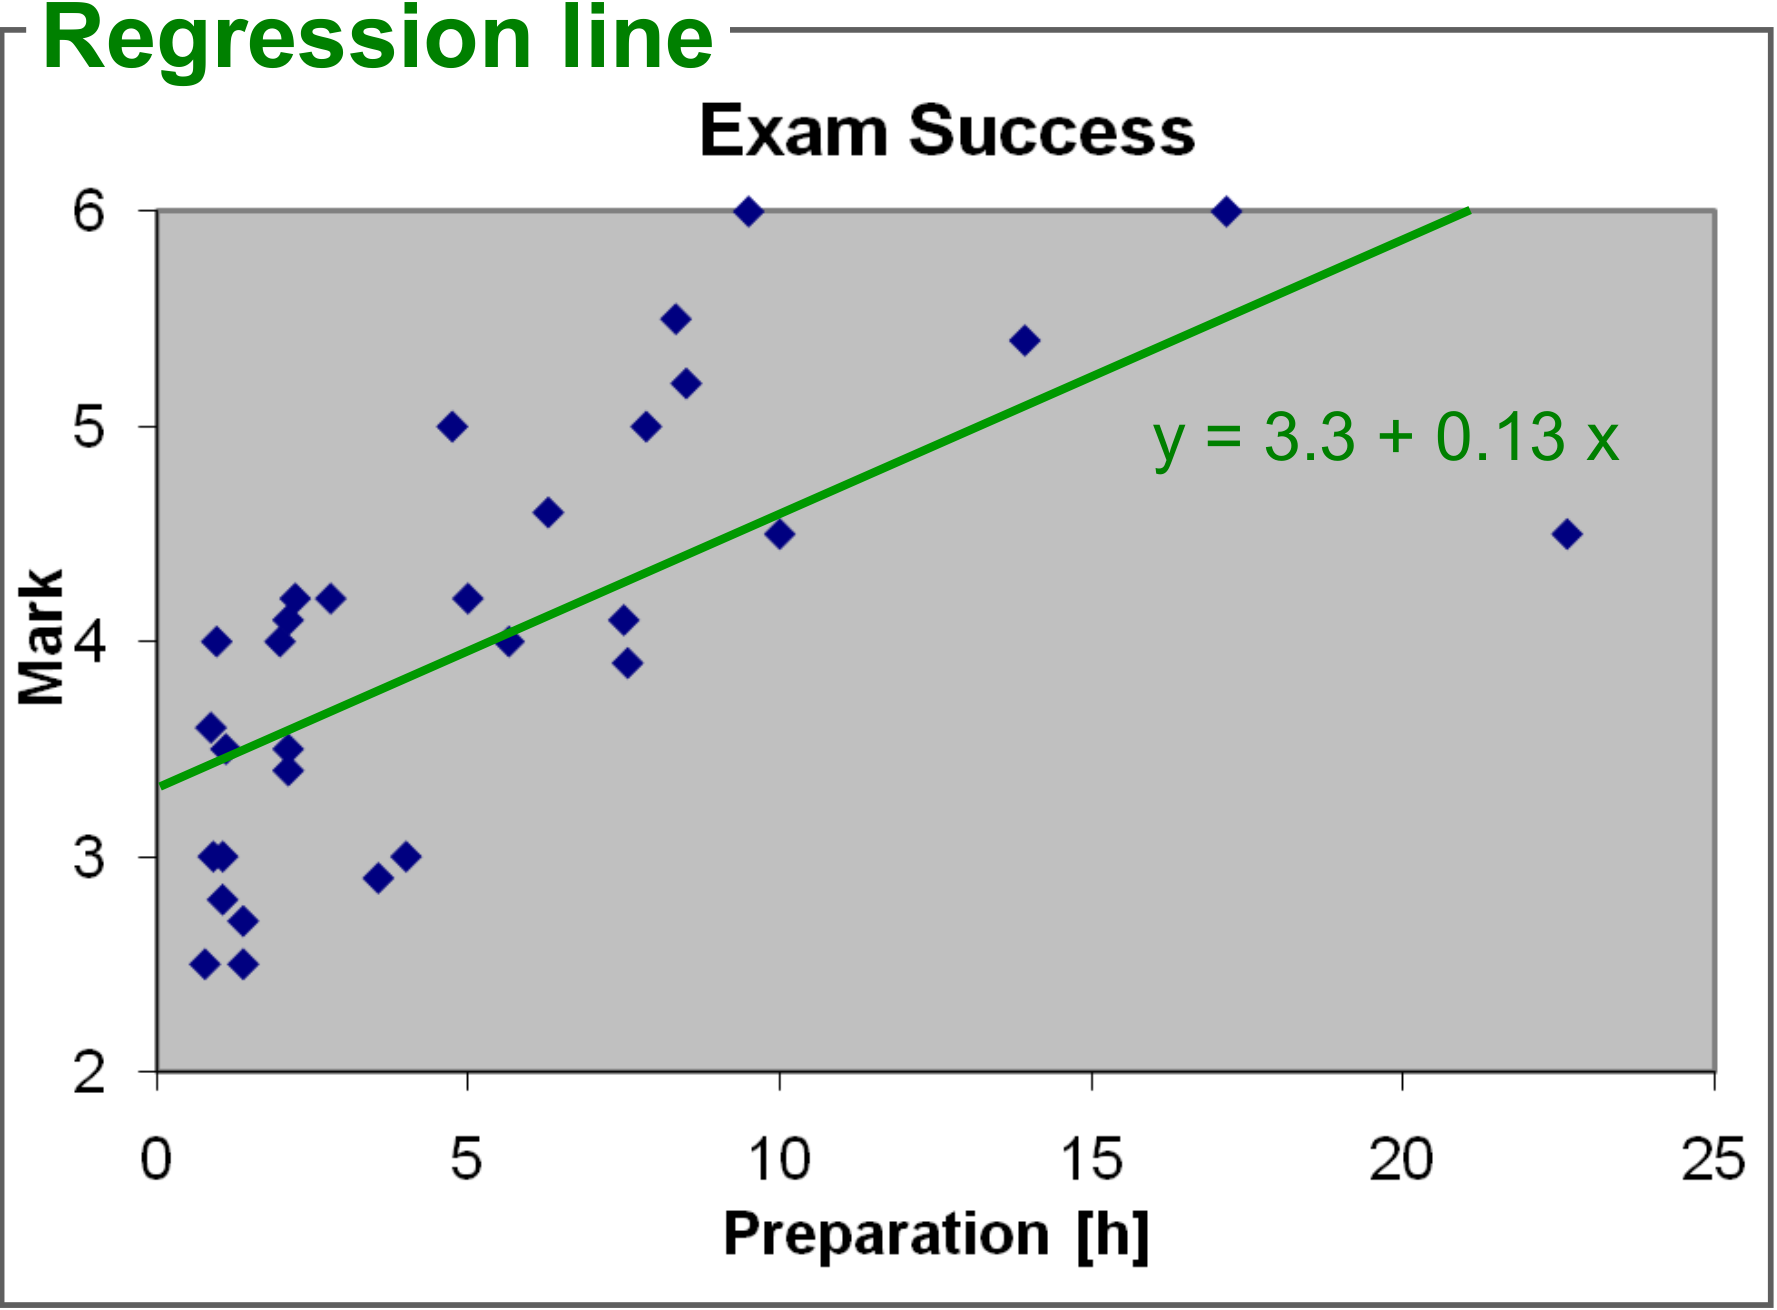
\includegraphics[width=.12\textwidth]{slides_images/data_reduction_regression_line}
%\end{center}
%\end{breakbox}



%\begin{breakbox}
%\boxtitle{Attribute Subset Selection Techniques:}
%Idea: explore the search space of attribute combinations for the most useful ones.
%\begin{itemize}
%	\item Stepwise Forward Selection
%	\item Stepwise Backward Elimination
%	\item Combination from both
%	\item Best-First: keeps calculation results for later recurrence
%	\item Beam Search: keeps constant number of most promising candidates
%	\item Genetic Algorithms: ''evolution'' by any number of permutations
%\end{itemize}
%\end{breakbox}


\begin{breakbox}
\boxtitle{Binning:}

Given: list with visitors' ages:

\begin{center}
7, 7, 8, 9, 10, 12, 13, 22, 22, 36, 38, 64
\end{center}

\begin{breakbox}
\boxtitle{Equidepth:}
Each bin should just hold 3 distinct values. $12/3=4$ since all bins should have the same size. Naming the bins is optional.

\begin{itemize}
	\item \textbf{Children:} $7 \leq age < 10$ with $7$ $7$ $8$ $9$
	\item \textbf{Youths:} $10 \leq age < 22$ with $10$ $12$ $13$ $22$
	\item \textbf{Adults:} $22 \leq age \leq 64$ with $22$ $36$ $38$ $64$
\end{itemize}

The objective is to sort the unknown instances. In the end, determining the bin boundaries is important, not the location of the training set's instances! So it does not matter that the two $22$ values are in different bins.
\end{breakbox}



\begin{breakbox}
\boxtitle{Equiwidth:}
Each bin should have the same interval width, again 3 bins.  Range from $7$ to $64 \implies$ $(64-7)/3=19$. One bin is exactly 19 years wide, except the last one which contains 20 items.

\begin{itemize}
	\item \textbf{Young:} $7 \leq age < 26$ with $7$ $7$ $8$ $9$ $10$ $12$ $13$ $22$ $22$
	\item \textbf{Youths:} $26 \leq age < 45$ with $36$ $38$
	\item \textbf{Adults:} $45 \leq age \leq 64$ with $64$	
\end{itemize}
\end{breakbox}

Grouping unknown instances:

\begin{tabular}{l|l|l}
\textbf{Age} & \textbf{equidepth} & \textbf{equiwidth} \\
\hline
8   & Children  & young     \\
22  & Adults    & young     \\
45  & Adults    & old       \\
6   & Children  & young     \\
70  & Adults    & old      
\end{tabular}

The two last entries are outside of the training set's value domain so the most fitting discrete value is assigned.
\end{breakbox}



\begin{breakbox}
\boxtitle{Confusion Matrix:}
ch=child, yth=youth, ad=adult

\begin{tabular}{l|l|l||l|l|l}
\textbf{G} & \textbf{Age} & \textbf{R} & \textbf{G} & \textbf{Age} & \textbf{R} \\
\hline
f & ch & MS   & f & yth & MS   \\
f & ch & WC   & f & yth & RC   \\
f & ch & WC   & f & yth & RC   \\
f & ch & WC   & m & yth & WC   \\
f & ch & MS   & m & yth & RC   \\
m & ch & MS   & m & yth & RC   \\
m & ch & WC   & m & ad & RC   \\
m & ch & WC   & m & ad & RC  
\end{tabular}

Given rules and which instances they classify:

\begin{enumerate}
	\item if age = \textbf{child} then \textbf{WC}
		\begin{itemize}
			\item 3 instances \textbf{MS} as \textbf{WC} (false)
			\item 5 instances \textbf{WC} as \textbf{WC} (true)
		\end{itemize}
	\item if age = \textbf{youth} and gender = \textbf{m} then \textbf{RC}
		\begin{itemize}
			\item 1 instance \textbf{WC} as \textbf{RC} (false)
			\item 2 instances \textbf{RC} as \textbf{RC} (true)
		\end{itemize}
	\item if age = \textbf{youth} and gender = \textbf{f} then \textbf{MS}
		\begin{itemize}
			\item 1 instance \textbf{MS} as \textbf{MS} (true)
			\item 2 instances \textbf{RC} as \textbf{MS} (false)
		\end{itemize}
	\item if age = \textbf{adult} then \textbf{RC}
		\begin{itemize}
			\item 2 instances \textbf{RC} as \textbf{RC} (true)
		\end{itemize}
\end{enumerate}

Confusion matrix formed by the above rules for the test set.
\begin{center}
	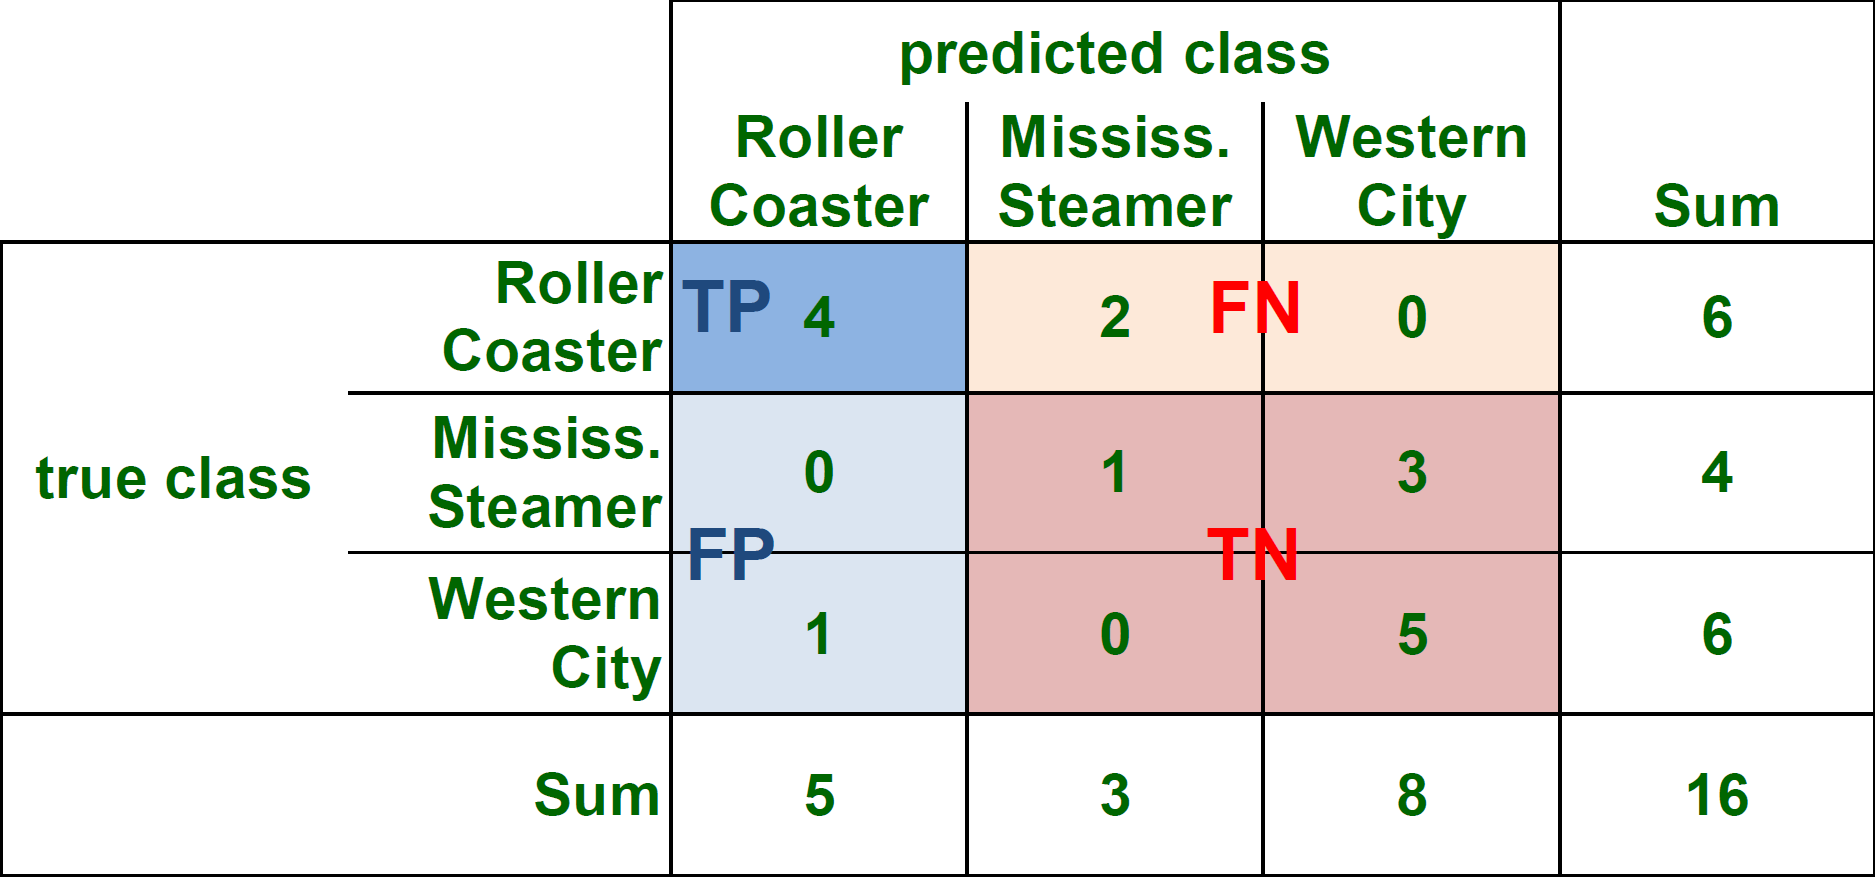
\includegraphics[width=.15\textwidth]{slides_images/confusion_matrix_theme_park}
\end{center}

Indicators:

\begin{itemize}
	\item True positives:
	\begin{itemize}
		\item target class, predicted correctly
		\item instances classified as ''RC'' \textbf{being indeed ''RC'': $2+2=4$}
	\end{itemize}
	\item False positives:
		\begin{itemize}
			\item target class predicted, actual class is different
			\item instances classified as ''RC'' but \textbf{being of some other class: $1$}		
		\end{itemize}
	\item True negatives:
		\begin{itemize}
			\item instances classified as not ''RC'' and \textbf{being indeed not ''RC'': $3 + 5 + 1 = 9$}
			\item contrast class, predicted correctly
		\end{itemize}
	\item False negatives: 
		\begin{itemize}
			\item constract class predicted, actual class different
			\item instances classified as not ''RC'' but \textbf{''RC'' though: $2$}
		\end{itemize}
	\item Precision = TP/(TP+FP) = $4/(4+1)=0.8$
	\item Recall = TP/(TP+FN) = $4/(4+2)=0.67$
\end{itemize}
\end{breakbox}



\begin{breakbox}
\boxtitle{F-Measure:}

Combines weighted average from both in just one indicator:

\begin{center}
$2 \cdot \frac{Precision \cdot Recall}{Precision + Recall} = \frac{2TP}{2TP + FN + FP} $ 
\end{center}

F-measure reaches its best value at 1 and worst at 0.
\end{breakbox}



\begin{breakbox}
\boxtitle{Cross-Validation:}

Trainings and test set are mostly limited available. Cross-validation helps to create more training data.

\begin{itemize}
	\item split training set in k partitions of roughly the same size
	\item build model k times
		\begin{itemize}
			\item each time another partition is taken as hold-out (i.e. test set)
			\item Hold out: keep a certain portion of available data for testing. The model is then built on the remaining data and tested with the hold out.
			\item the remaining partitions together are the training set
		\end{itemize}
	\item image with 3-fold ''cross-validation'' 
\end{itemize}

\begin{center}
	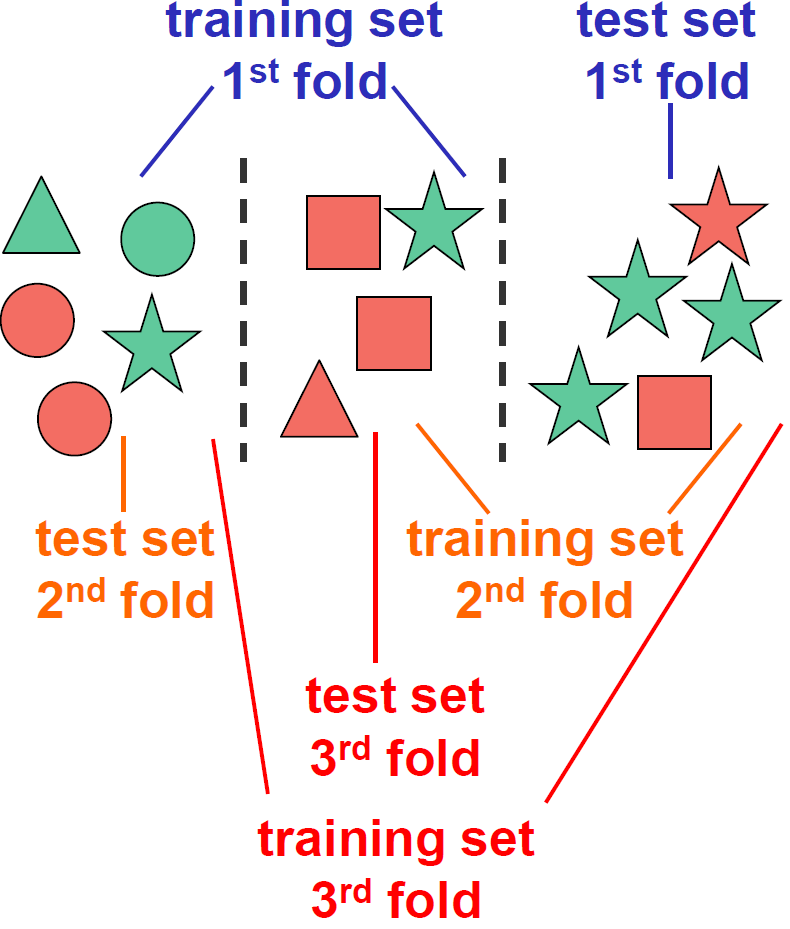
\includegraphics[width=.065\textwidth]{slides_images/cross_validation}
\end{center}


The \textbf{repeated} crosss-validation repeat the cross-validation n times. Each time the data is split into k different partitions to make sure not being misled by some accidental odd distribution of data. Best practice: n=10 so 100 different models are ''learned''. Image with n=3.

\begin{center}
	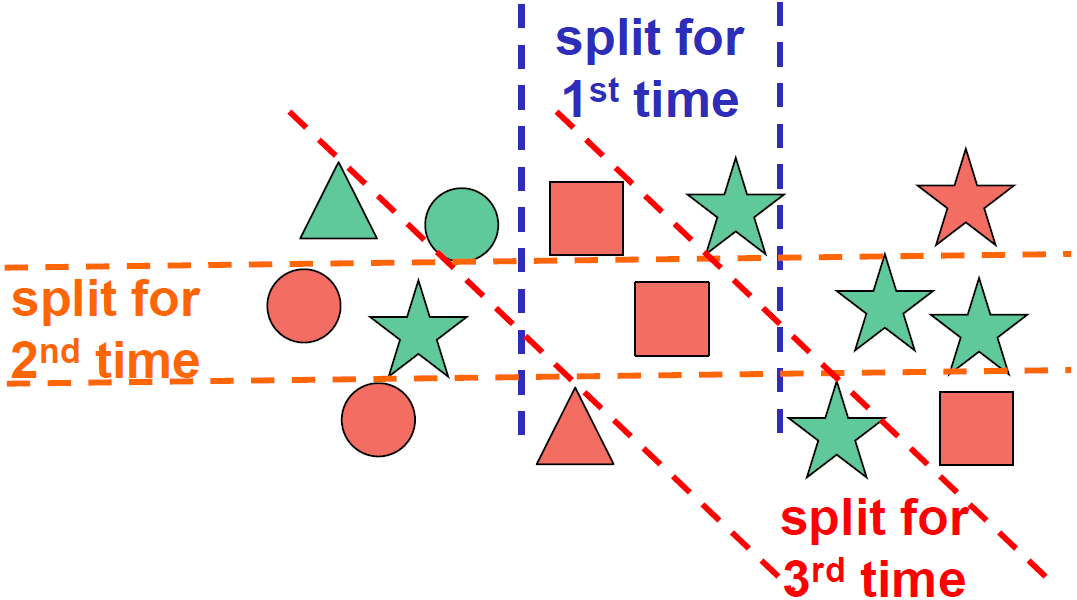
\includegraphics[width=.08\textwidth]{slides_images/repeated_cross_validation}
\end{center}

\textbf{Stratified} (=geschichtet) cross-validation: Class distribution within training and test sets impacts prediction quality. So the overall class distribution is to be maintained in each partition for every split.

\begin{center}
	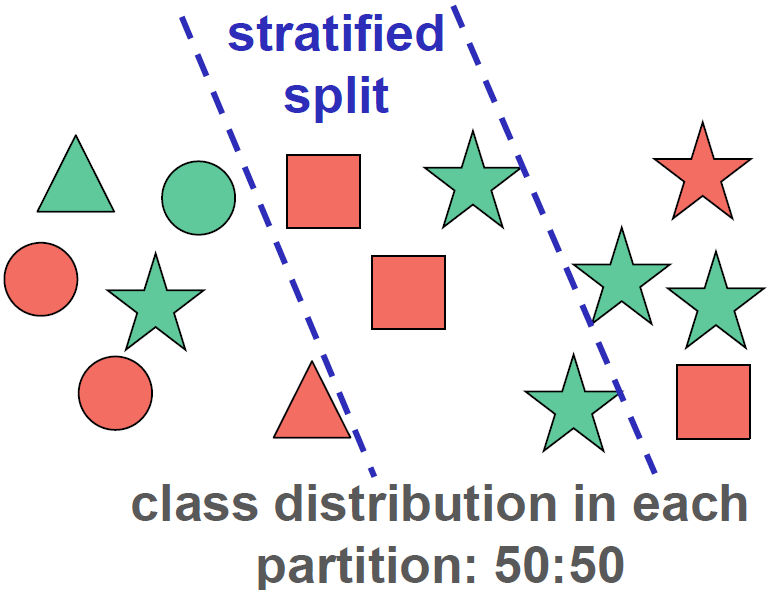
\includegraphics[width=.07\textwidth]{slides_images/stratified_cross_validation}
\end{center}
\end{breakbox}



\begin{breakbox}
\boxtitle{Chi squared test}

Proof or disproof that two variables are independent. Correlation/lift only measures linear dependencies, $\chi ^2$ also non-linear. If error surmounts a given threshold then there is a dependency.
\begin{center}
	$\chi ^2 = \sum_{i}{} \sum_{j}{} \frac{(observed_{ij} - expected_{ij})^2}{expected_{ij}}$
\end{center}

\begin{center}
	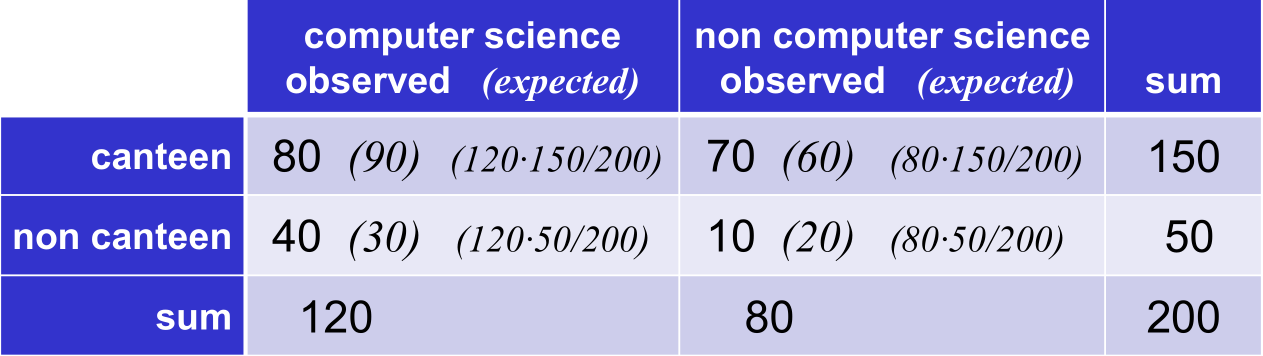
\includegraphics[width=.15\textwidth]{slides_images/chi_squared_test_example}
\end{center}

\begin{center}
	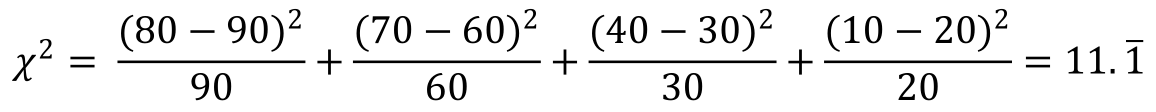
\includegraphics[width=.15\textwidth]{slides_images/chi_squared_test_canteen_numbers}
\end{center}

For a significance level of 0.001 (probability of error is 1 per mille and for a degree of freedom=1 (applies for 2 classes per attribuite). This results in a max. treshold $\chi^2 = 10.83$ so the above attributes ''going to canteen'' and ''studying cs'' are dependent.
\end{breakbox}



\begin{breakbox}
\boxtitle{Cluster Quality Measures:}

\begin{itemize}
	\item Compactness
		\begin{itemize}
			\item instances in a distinct cluster are close to each other
			\item = itraclass similarity is high		
	\end{itemize}				
	\item Separation
		\begin{itemize}
			\item clusters are well apart from each other
			\item = interclass dissimilarity is high
		\end{itemize}
\end{itemize}

\textbf{Compactness:} Measuring distances inside clusters with $x_i$: instance i of a cluster, $n$: number of instances in a cluster, $c$: cluster center:
\begin{itemize}
	\item Cluster density
		\begin{itemize}
			\item average distance of instances in one cluster
			\item $\frac{1}{n} \cdot \sum_{1}^{n}(x_i - c)$ 
		\end{itemize}
	\item Variance
		\begin{itemize}
			\item if low: instances concentrate around center
			\item $\sum_{1}^{n}(x_i - c)^2$
		\end{itemize}
	\item Average variance
		\begin{itemize}
			\item takes into account cluster size
			\item $\frac{1}{n} \cdot \sum_{1}^{n}(x_i - c)^2$ 
		\end{itemize}
\end{itemize}

\textbf{Separation:} Measuring distance between clusters:
\begin{itemize}
	\item Single linkage: distance between the two closest instances from two different clusters
	\item Complete linkage: distance between two most distant instances
	\item Average linkage: average distance between all instances (each instance of one cluster to every instance from other one)
	\item Distance of cluster centers
\end{itemize}

\begin{center}
	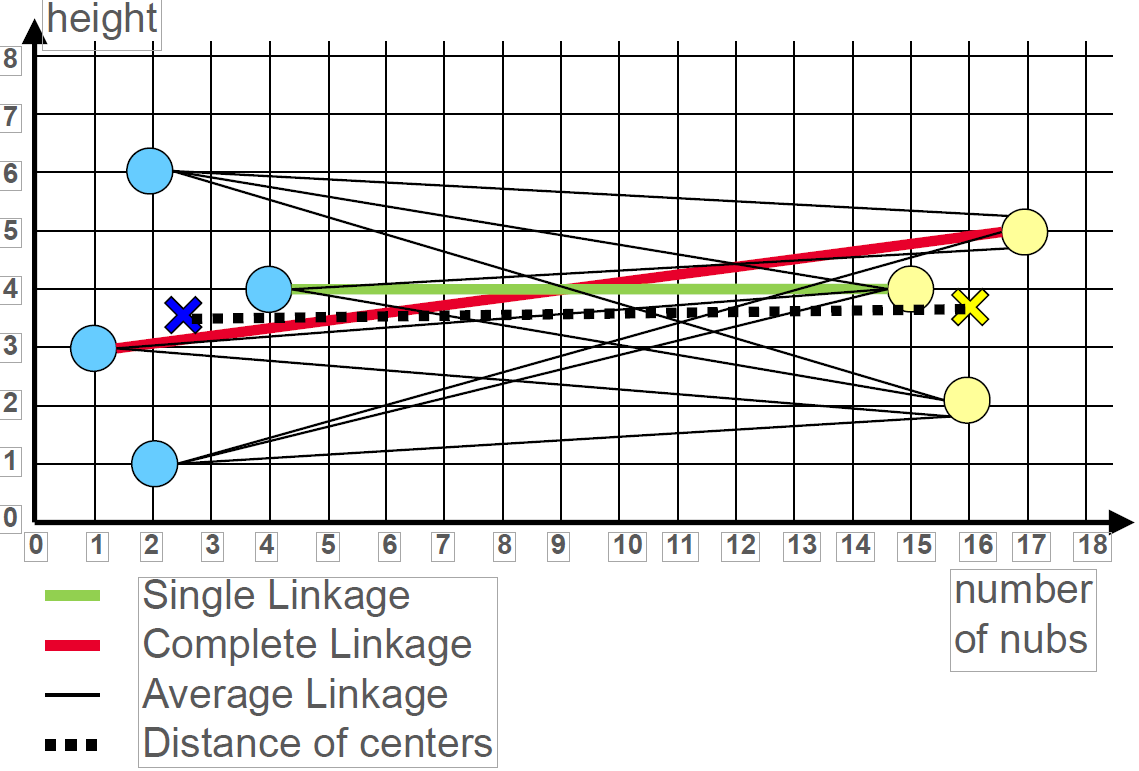
\includegraphics[width=.15\textwidth]{slides_images/cluster_distance_measurements_separation}
\end{center}

\end{breakbox}

